\subsection{Reinforcement learning \label{RL}}

In the field of machine learning, the subfield of reinforcement learning
deals with training agents in how to behave in an environment through
trial and error. The environment typically consists of a set of states that cover all
scenarios the agent can encounter. The agent then has a set of actions
that it can use to make transitions between the states. 
The reinforcement learning methods relates somewhat 
to supervised models.
In supervised learning, every decision is tied to a predefined value
that defines how desirable the given action is. This way, in supervised learning,
the agent will always at any point have very detailed feedback signals from its actions.
In the context of actions and state transitions, an agent that learns through
supervised learning will for every action taken know the absolute consequence
immediately after committing it.
Reinforcement learning is in many ways similar to supervised learning. 
The main difference between the two models is that agent does not receive 
an immediate response to its actions. Instead, the agent will receive a reward
when reaching certain states. The objective of the agent is then to
accumulate as much reward as possible. This differs from supervised learning
as the agent cannot know if reaching high amounts of intermediate reward in the next state
will cause negative consequences in the future. Thus, the only decisive 
feedback given to the agent about its overall performance is 
how much cumulative reward it achieved at the end of a game.
In the game of Tetris, the reward is a direct mapping to 
the score achieved by the agent.
As a simple example of how these two learning models apply, consider 
the simple game of
Tic Tac Toe. If supervised learning
is applied, the playing agent will for each move in the game know
if the move was considered desirable or not. 
In reinforcement learning however, the only feedback the agent receives
is whether the games ended in a win, draw or a loose. Hence, the agent
cannot rely on signals during the game to adjust its strategy.

\begin{figure}[H]
\begin{center}
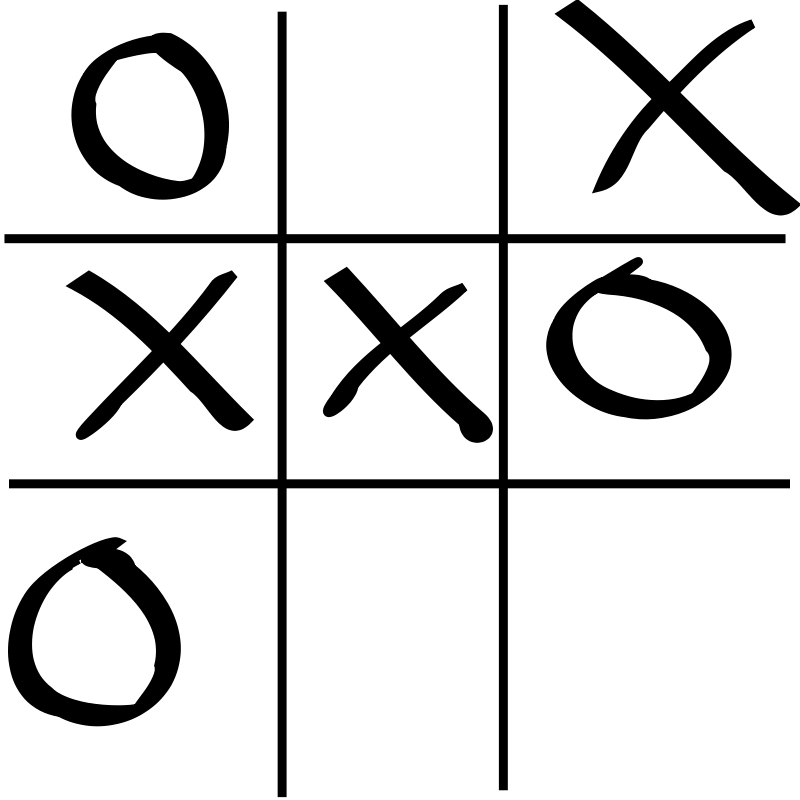
\includegraphics[scale=0.2]{img/tic_tac_toe}
\end{center}
\caption{Illustration of a Tic Tac Toe board}
\end{figure}


Often in the case of games, the 
time frame naturally falls into playthroughs in which the 
goal of the agent is to accumulate as much reward as possible 
before the game ends.
When the agent interacts 
with the environment, it uses a predefined set of actions
that each alters the state of the environment. In the case of 
Tic Tac Toe, the environment is the current state of the game, 
in terms of which markers are occupying spaces on the board.
The actions are the options to place a marker
on an empty space.
When deciding which action to carry out, the agent will use
a policy that maps the state of the environment to an action.
In Tic Tac Toe, a policy might be a table that has an entry for each possible
state of the board that maps to where the agent should place its marker.
The goal of the agent is then to choose a policy that maps states to actions 
in a way that
gives the highest possible cumulative reward at the end of a playthrough. 
Rewards in states can be negative and cause a 'penalty' to the agent if it reaches
such state. However, in the case of Tetris the agent cannot lose score,
and will therefore never be directly  penalized.
Games often have a terminal state at which the game ends, which is 
also the case for Tetris and Tic Tac Toe. It's easy to see how the
Tic Tac Toe cannot last forever as it has 9 spaces, and for each turn in the game,
a space is occupied. However, the reason for why Tetris cannot play forever
lies within the fact that there exists a sequence of pieces that will
with certainty cause the player to lose, and if the player plays for 
long enough, this sequence will eventually occur. Thus, the agent must
attempt to acquire as much reward as possible before reaching the terminal 
state. 
When the agent chooses an action it cannot necessarily know what state
the action leads to, and in games this uncertainty is often present.
In Tic Tac Toe, the action taken by the agent will always with certainty 
lead to a known state, namely the board configuration where the marker is placed.
However, in Tetris, part of the state is the piece that is currently falling.
Thus, when the agent chooses a place to drop the piece, it has full control
over where to drop it, yet it cannot decide what the next active piece is.
As there are 7 different piece
types in Tetris, each action can lead to 7 other states, each with a predefined probability.
It should also be noted that these probabilities for the individual transitions
must remain fixed across the entire playthrough of the game \citep{Carr}.
To find the best policy, there are a number of methods to pick from,
and the most obvious is a full traversal of the entire state space.
If one can afford to compute all rewards acquired from all possible 
actions in all possible states, one can choose the policy 
that gives the best expected cumulative reward. However, if the state space is
large, such computations become infeasible. The state space in Tetris
is indeed far too large to comprehensively traverse.
Due to this, one must use other means of discovering good policies.
The methods used in reinforcement learning 
specify how the agent should change its policy according to 
results from earlier playthroughs, and the specific methods used in
the context of Tetris is explained in further detail in later sections.


